\section{Nasazení a provoz projektu}
\label{sec:deployment-running}

Tato kapitola je věnována nasazení a provozu projektu \bso. Popisuje volbu hostingové služby a důvody k ní vedoucí, serverovou architekturu a obsahuje také poznatky a překonané problémy, které v průběhu nasazování projektu vznikli.

\subsection{Hostingová služba}
\label{sub:hosting}

Při navrhování projektu \bso byly zvažovány služby Amazon AWS\cite{amazon-aws}, Microsoft Azure\cite{ms-azure} a cloudem společnosti Digitalocean\cite{digitalocean}. Všechny tři služby poskytují velké množství pokročilých funkcí pro vývoj a provoz webových aplikací. 

Nakonec byl pro většinu funkcí zvolen cloud společnosti Digitalocean, jelikož má ze všech tří poskytovatelů nejjednodušší správu a finanční politiku, je přesně uvedeno za co platíte a neexistují žádné skryté limity a kvóty. Mezi další výhody cloudu Digitalocean patří vysoký výkon a velmi příznivé ceny.\cite{digitalocean-advantages}

Pro další funkcionality jako ukládání souborů a zasílání emailů byly využity služby Amazon S3\cite{amazon-s3} a Amazon SES\cite{amazon-ses}. Důvody pro toto rozhodnutí byly bezkonkurenční ceny a integrace s použitými technologiemi, hlavně \gls{framework}em \nameref{subsub:laravel}.


\begin{figure}[!ht]
\centering
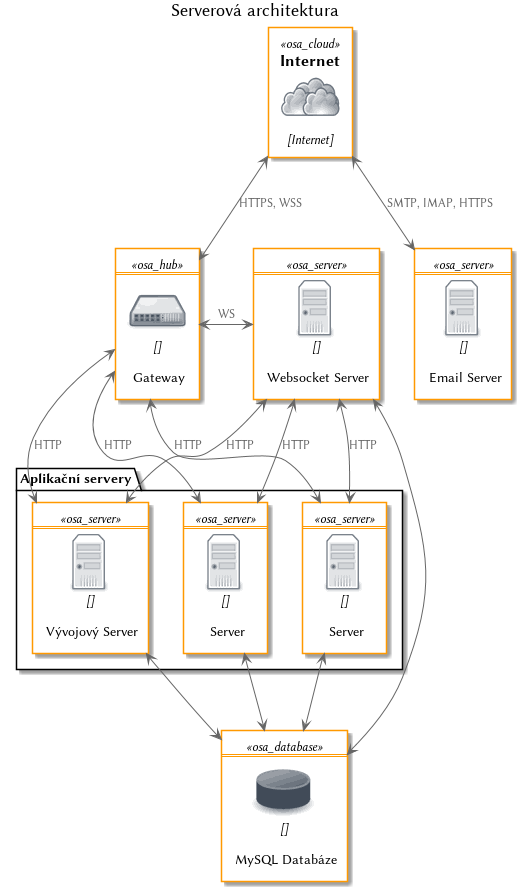
\includegraphics[width=11cm]{img/serverova-architektura.png}
\caption{Serverová architektura projektu \bso}
\label{fig:servery}
\end{figure}

\clearpage

\subsection{Serverová architektura}

\emptyLine

\begin{displayquote}
Internet je divokým a nebezpečným místem\cite{internet-is-dangerous-place}.
\end{displayquote}

\begin{displayquote}
\acrlong{sw} a \acrlong{hw} je nespolehlivý, chyba není výjimka ale pravidlo\cite{failure-is-rule-not-exception}.
\end{displayquote}

\emptyLine

Podle těchto dvou faktů musíme řídit svůj návrh serverové infrastruktury.  Musíme tedy vytvořit serverovou infrastrukturu, která je odolná, bezpečná a škálovatelná.

Z hlediska bezpečnosti můžeme rozdělit servery projektu \bso na dvě skupiny: okrajové servery a interní servery.

Okrajové servery mají za úkol komunikaci s Internetem. Jedná se o několik přesně definovaných míst, skrze něž prochází všechna komunikace určená mimo naši infrastrukturu.

Jednou z hlavních výhod tohoto přístupu je možnost využívat uvnitř naší infrastruktury nešifrované protokoly jako \acrshort{http} a provádět jejich zašifrování pouze na těchto dedikovaných okrajových serverech. Tyto nešifrované protokoly jsou výkonnější a jednodušší než jejich šifrované varianty\cite{http-faster-https}. Z důvodu bezpečnosti je ale není možné použít pro Internetovou komunikaci.

Z pohledu resilience, obrany proti výpadku, jsou nejdůležitějšími opatřeními replikace a \hyperref[sub:load-balancing]{load-balancing} klíčových částí. Využíváme proto \hyperref[sub:load-balancing]{load balancery} a \hyperref[subsub:managed-databases]{spravované databáze}, u kterých neznamená výpadek jednoho stroje nedostupnost celé aplikace.


\subsection{Postup nasazení aplikace}
\label{sub:deployment}

Prvním krokem je provize serveru. Jelikož projekt \bso obsahuje pouze malý počet serverů, bylo možné všechny servery nakonfigurovat a vytvořit přímo z ovládacího panelu Digitalocean.

Poté co jsou servery vytvořeny přejdeme ke konfiguraci samostatných serverových rolí. Každá serverová role vyžaduje separátní konfiguraci a specifický software, aby mohla svou funkci vykonávat.

Dalším krokem je vytvoření obrazů disků nakonfigurovaných serverů, abych mohl rychle a jednoduše vytvářet další servery těchto rolí. Pro každou serverovou roli byl vytvořen seznam parametrů, které je po vytvoření serveru z obrazu disku nutné upravit. U aplikačních serverů je například nutné upravit \acrshort{ip} adresu, na které má webový server naslouchat pro nová připojení. 

Posledním krokem je nastavení příslušných \acrshort{dns} záznamů a získání \acrshort{ssl} certifikátů.

\subsection{Nasazování aktualizací aplikace}
\label{sub:update-deployment}

První přístup nasazování aktualizací, který byl na nasazování projektu \linebreak
\bso využit, byl založený na Github Actions\cite{github-actions}. Github Actions je \gls{ci-cd} mechanismus založený na spouštění kódu v závislosti na událostech verzovacího systému Git\cite{git}. Využíván byl SSH for Github Actions\cite{ssh-for-github-actions}, pro automatické nasazování při commitu do dedikované větve.

Tento přístup má několik problémů. Hlavním problémem je fakt, že pro každý přidaný cílový server je zapotřebí vytvořit novou konfiguraci. Když vysazovací akce selže, je těžké najít příčinu, jelikož výpisy Github Actions jsou nepřehledné a zaměňují \acrshort{stdout} a \acrshort{stderr}. Posledním velkým problémem tohoto přístupu je, že pro spuštění vysazení je zapotřebí změna v kódu aplikace.

Tyto problémy jsem vyřešil použitím Laravel Envoy\cite{laravel-envoy}. Laravel Envoy využívá konfigurační soubory v jazyce \acrshort{php} pro provádění dávek akcí na skupině serverů zároveň. Pokud je zapotřebí přidat nový server, stačí přidat jeho \acrshort{ip} adresu do seznamu serverů a Laravel Envoy automaticky provede všechny potřebné akce. Další velkou výhodou je absence nutnosti ukládat \acrshort{ssh} klíče na serveru třetí strany. Pro zopakování vysazení stačí pouze znovu spustit Laravel Envoy.